\documentclass{TIJMUjiaoanLL}
\pagestyle{empty}


\begin{document}


%课程名称
\kecheng{Linux系统概论}
%课程内容
\neirong{常用Linux命令\ /\ 第6章}
%教师姓名
\jiaoshi{伊现富}
%职称
\zhicheng{讲师}
%教学日期(格式:XXXX年XX月XX日XX时-XX时)
\riqi{2018年5月28日10:00-12:00}
%授课对象(格式:XXX系XXXX年级XX班(硕/本/专科))
\duixiang{生物医学工程与技术学院2016级生信班(本)}
%听课人数
\renshu{28}
%授课方式
\fangshi{理论讲授}
%学时数
\xueshi{2}
%教材版本
\jiaocai{Unix入门经典,第1版}


%教案首页
\firstHeader
\maketitle
\thispagestyle{empty}

\mudi{
\begin{itemize}
  \item 掌握Linux命令的基本格式,查找命令相关信息的各种方法,基本的通配符,输入输出重定向的方法,管道的使用,Linux的常用命令。
  \item 熟悉常用的转义符,命令置换的方法,熟悉命令的自动补全。
  \item 了解命令的历史及别名,命令连接符,常用的终端快捷键。
  \item 自学Linux各种命令的使用方法及常用选项。
\end{itemize}
}

\fenpei{
\begin{itemize}
  \item (5')引言与导入:简要介绍命令是什么,总结进入命令行界面的方法。
  \item (10')命令的剖析:讲解Linux命令的基本格式。
  \item (10')查找命令的相关信息:介绍查找命令相关信息的四种方法。
  \item (25')命令的修改:介绍常用的通配符、转义符和命令置换的方法,讲解输入输出重定向的方法和管道的使用。
  \item (35')常用命令汇总:汇总介绍目录操作、文件操作、权限管理等常用的命令,讲解ls、mv、rm、wc、sort、uniq、cut、tar等重要命令的常用选项。
  \item (10')命令使用技巧:介绍自动补全,命令历史、别名、连接符和终端快捷键等使用技巧。
  \item (5')总结与答疑:总结授课内容中的知识点与技能,解答学生疑问。
\end{itemize}
}

\zhongdian{
\begin{itemize}
  \item 重点:Linux命令的基本格式,查找命令相关信息的方法,Linux的常用命令。
  \item 难点:常用通配符,输入输出重定向,管道的使用。
  \item 解决策略:通过实例讲解与操作演示帮助学生理解、记忆。
\end{itemize}
}

\waiyu{
  \vspace*{-10pt}
  \begin{multicols}{2}
    参数(argument)

    选项(option)

    元字符(metacharacter)

    通配符(wildcard)

    标准输入(STDIN,standard input)

    标准输出(STDOUT,standard output)

    标准错误(STDERR,standard error)

    管道(pipe)

  \end{multicols}
  \vspace*{-10pt}
}

\fuzhu{
\begin{itemize}
  \item 多媒体:Linux命令的基本格式,各种通配符的含义,常用的转义符。
  \item 板书:输入输出重定向的方法,管道的使用,各种命令连接符的含义。
  \item 演示:Linux常用命令及其常用选项的使用,各种命令使用技巧。
\end{itemize}
}

\sikao{
  \vspace*{-10pt}
  \begin{multicols}{2}
  \begin{itemize}
    \item Linux命令由哪几部分构成?
    \item 查找命令相关信息的方法有哪些?
    \item 列举三个常用的通配符并举例说明。
    \item 如何进行输入输出的重定向?
    \item 命令置换的方法有哪些,举例说明。
    \item 列举几个常用的命令及其常用选项。
    \item 列举命令使用技巧并进行说明。
  \end{itemize}
  \end{multicols}
  \vspace*{-10pt}
}

\cankao{
\begin{itemize}
  %\item (美)Paul Love,Joe Merlino\ 等著,张楚雄,许文昭\ 译。Unix入门经典,清华大学出版社,2006。
  \item (美)Harley Hahn\ 著,张杰良\ 译。Unix \& Linux大学教程,清华大学出版社,2010。
  \item 鸟哥\ 著,王世江\ 改编。鸟哥的Linux私房菜——基础学习篇(第三版),人民邮电出版社,2010。
  \item 维基百科等网络资源。
\end{itemize}
}

\firstTail


%教案续页
\newpage
\otherHeader

\begin{enumerate}
  \item 引言与导入(5分钟)
    \begin{itemize}
      \item 命令
      \begin{itemize}
\parpic[fr]{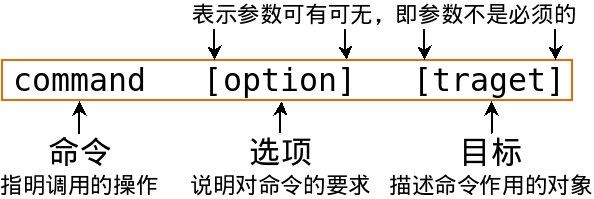
\includegraphics[width=9cm,height=2.3cm]{c4.command.png}}
        \item 可执行的程序,使用户能够要求机器执行某种操作
        \item 有时是shell的内置功能
        \item 有时是单独的程序
      \end{itemize}
      \item 进入命令行界面
	\begin{itemize}
	  \item 远程登录:ssh USER@HOSTNAME
	  \item 本地桌面
	    \begin{itemize}
	      \item 开机直接进入:不安装图形界面
	      \item 虚拟终端(从图形界面完全切换到命令行界面):Ctrl+Alt+F[1-6]
	      \item 终端模拟器(在图形界面中使用命令行):打开Terminal/终端
	    \end{itemize}
	\end{itemize}
    \end{itemize}

  \item \textcolor{red}{\textbf{【重点】}}命令的剖析(10分钟)\textcolor{red}{(讲解实例,与个性化点餐相类比)}
    \begin{enumerate}
\parpic[fr]{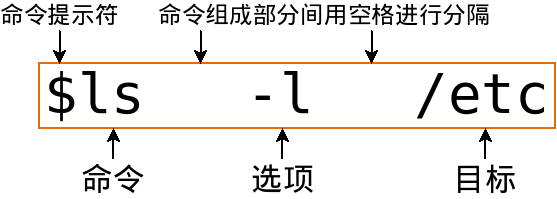
\includegraphics[width=9cm,height=2.6cm]{c4.command.ls.png}}
      \item Linux命令的基本格式
	\begin{itemize}
	  \item Linux命令 = 命令 + [参数]
	  \item 命令参数 = [选项] + [目标]
	  \item 分隔符:空格
	\end{itemize}
      \item 补充说明
	\vspace*{-10pt}
	\begin{multicols}{2}
	\begin{itemize}
	  \item 命令名与操作一致\textcolor{red}{(ls: list)}
	  \item 命令的默认行为\textcolor{red}{(ls)}
	  \item 参数影响输出格式和操作\textcolor{red}{(-l /etc)}
	  \item 目标提供处理目标\textcolor{red}{(/etc)}
	  \item 有些命令需要多个目标\textcolor{red}{(cp OLD NEW)}
	  \item 命令有独特的选项\textcolor{red}{(ls -l)}
	  \item 选项在一个或两个连字符后\textcolor{red}{(-a = -\ -all)}
	  \item 选项可以独立或是合并\textcolor{red}{(-a -l = -al)}
	\end{itemize}
      \end{multicols}
	\vspace*{-10pt}
    \end{enumerate}

  \item \textcolor{red}{\textbf{【重点】}}查找命令的相关信息(10分钟)\textcolor{red}{(讲解、演示实例)}
    %\vspace*{-10pt}
    %\begin{multicols}{2}
      \begin{itemize}
\parpic[fr]{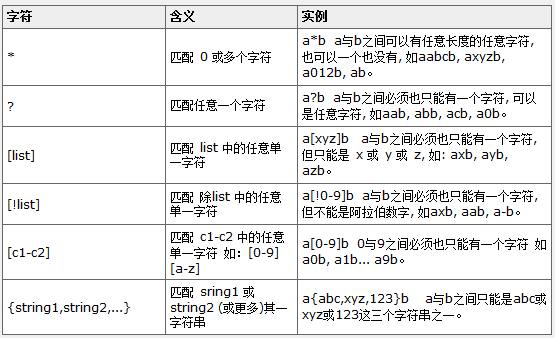
\includegraphics[width=10cm,height=7cm]{c4.metacharacter.png}}
	\item man CMD:联机帮助页(详细)
	\item info CMD:信息帮助页
	\item CMD -\ -help:帮助信息(简单)
	\item apropos KEY:查找文件
	\item whereis CMD:查找软件包
      \end{itemize}
    %\end{multicols}
    %\vspace*{-10pt}

    \item \textcolor{red}{\textbf{【难点】}}命令的修改(25分钟)\\ \textcolor{red}{(讲解、演示实例)}
    \begin{enumerate}
      \item 通配符
	\begin{itemize}
	  \item *.doc: 所有word文档
	  \item *.t[ex]*: 所有文本文件
	\end{itemize}
      \item 转义符
	\begin{itemize}
	  \item \verb|''|:硬转义
	  \item \verb|""|:软转义
	  \item \verb|\|:转义
	\end{itemize}
      \item 输入输出重定向
        \vspace*{-10pt}
	\begin{figure}[h]
	  \centering
	  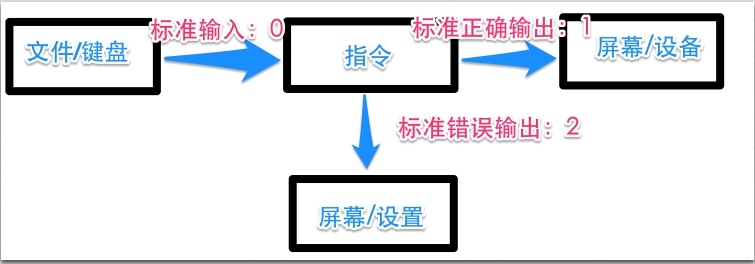
\includegraphics[width=7.5cm]{c4.io.01.jpg}
	  \quad
	  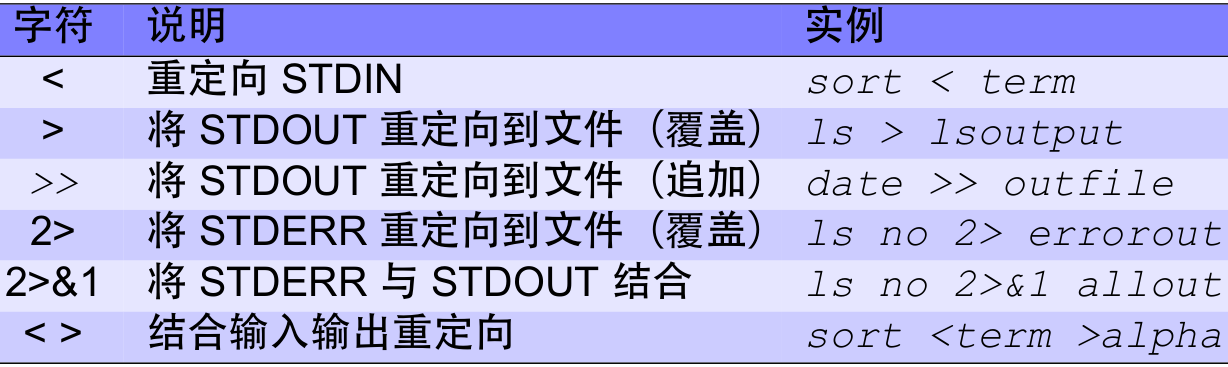
\includegraphics[width=9.3cm]{c4.io.png}
	\end{figure}
        \vspace*{-10pt}

\otherTail
\newpage
\otherHeader

      \item 管道\textcolor{red}{(与工作流水线相类比;实例:先复制后粘贴)}
\parpic[fr]{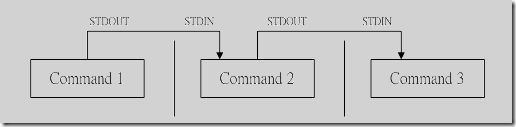
\includegraphics[width=8cm]{c4.pipe.png}}
	\verb=|=,一个操作符,把输入和输出重定向结合在一起,将一个命令的输出立即作为另一个命令的输入。\textcolor{red}{(ls -l /etc | less)}
      \item 命令置换
	\\ 将一个命令的输出作为另一个命令的参数的方法。
	\begin{itemize}
	  \item \verb|$()|: \verb|ls $(pwd)|
	  \item \verb|``|: \verb|ls `pwd`|
	  %\item \verb|${}|: \verb|ls ${pwd}|
	\end{itemize}
    \end{enumerate}

  \item \textcolor{red}{\textbf{【重点】}}常用命令汇总(35分钟)\textcolor{red}{(演示常用命令及其选项的操作)}
    \begin{enumerate}
      \item 目录操作:pwd,ls,cd,mkdir,rmdir,tree,du
      \item 文件操作:file,cat,touch,cp,mv,rm,ln,head,tail,more,less,wc,sort,uniq,cut,tee
      \item 权限管理:chown,chgrp,chmod,useradd,usermod,userdel,groupadd,groupmod,groupdel,passwd,w,who,whoami,finger,umask
      \item 系统导航:which,whereis,find,locate,updatadb,alias,df,mount,date,cal
      \item 进程管理:top,ps,pstree,kill,killall,uptime,uname,free,jobs,bg,fg,cron,at
      \item 压缩解压:tar,gzip,gunzip,bzip2,bunzip2,zip,unzip
      \item 关机重启:shudown,reboot,halt,poweroff
      \item 获取帮助:man,info,apropos,whatis,-\ -help
      \item 命令详解:ls,cat,rm,wc,sort,uniq,cut,tar等
    \end{enumerate}

  \item 命令使用技巧(10分钟)
    \vspace*{-10pt}
    \begin{multicols}{2}
    \begin{enumerate}
      \item 自动补全:Tab
      \item 历史命令:history,上下方向键
      \item 命令别名:alias,unalias
      \item 命令连接符
	\begin{itemize}
	  \item ;:命令顺序执行
	  \item \&\&::逻辑与关系
	  \item ||:逻辑或关系
	\end{itemize}
      \item 后台运行:CMD \&,nohup CMD \&
      \item 终端快捷键
	\begin{itemize}
	  \item Ctrl+L:终端清屏
	  \item Ctrl+C:终止命令
	  \item Ctrl+D:注销会话
	  \item Ctrl+R:搜索命令历史
	  \item ……
	\end{itemize}
    \end{enumerate}
    \end{multicols}
    \vspace*{-10pt}

  \item 总结与答疑(5分钟)
    \begin{enumerate}
      \item 知识点
	\begin{itemize}
	  \item Linux命令的基本结构:命令、参数(选项、目标)
	  \item 查找命令相关信息的方法:man、info、\verb|--help|、apropos
          \item 命令的修改:元字符、输入输出重定向、管道、命令置换
          \item 目录和文件操作、权限管理、系统导航、压缩解压等常用命令
          \item 命令使用技巧:补全、历史、别名、连接符、后台运行、快捷键
	\end{itemize}
      \item 技能
	\begin{itemize}
          \item 常用命令及其选项的使用
          \item 命令的修改
          \item 命令的使用技巧
	\end{itemize}
    \end{enumerate}

\end{enumerate}

\otherTail


\end{document}

